\section{Introduction}


\subsection{The model}
We study a uniform directed graph (or digraph) with a random degree sequence. We consider $n$ vertices, to each of which we assign an in-degree and an out-degree. The degree tuples are independent and identically distributed. Let $\mathbf{D}=(D^-,D^+)$ be a random variable in $\N\times \N$ with this distribution, and for each $i\in [n]$, let $\mathbf{D}_i=(D^-_i,D^+_i)$  be the in- and out-degree of vertex $i$. In order for a graph with this degree sequence to exist, we require that $\sum_{i=1}^n D^-_i=\sum_{i=1}^n D^+_i$, so we will condition on this event. We are interested in the limit under scaling of the strongly connected components as $n\to \infty$.  \\

We require the degree distribution to satisfy the following properties. \myworries{Change to notation Zheneng}


\begin{enumerate}
    \item \label{cond.mu}$\E[D^+]=\E[D^-]=\E[D^-D^+]$
     \item \label{cond.gamma}$\E\left[(D^-)^3\right]<\infty$
    \item \label{cond.rho} $\E\left[(D^+)^2 D^-\right]<\infty$
      \item \label{cond.iota} $\E\left[D^+(D^-)^3\right]<\infty$
      \item $\E\left[(D^+)^3D^-\right]<\infty$
\end{enumerate}

We define the following parameters, that will determine the behaviour of the strongly connected components in the limit.
\begin{enumerate}
    \item $\mu:=\E[D^-]=\E[D^+]=\E[D^-D^+]$
    \item $\nu_-:=\frac{\E[(D^-)^2]-\mu}{\mu}$ 
    \item $\sigma_-:=\left(\frac{\mu\E[(D^-)^3]-\E[(D^-)^2]^2}{\mu^2}\right)^{1/2}$ 
    \item $\sigma_+:=\left(\frac{\E[D^-(D^+)^2]-\mu}{\mu}\right)^{1/2}$ 
    \item $\sigma_{-+}:=\frac{\E[(D^-)^2D^+]-\E[(D^-)^2]}{\mu}$ 
\end{enumerate}
% \begin{remark}
% Conditions \ref{cond.beta} and \ref{cond.gamma} ensure that the Central Limit Theorem applies to the fluctuations of the first explored in-degrees around their mean. Condition \ref{cond.critical} ensures that the branching process corresponding to the depth-first exploration (i.e. the exploration of the out-components) is critical. Condition \ref{cond.rho} ensures that this branching process has Brownian scaling. Condition \ref{cond.tau} ensures that the covariance of the in- and out-degrees that are discovered first is finite. Condition \ref{cond.iota} ensures that the strongly connected components are $3$-regular. 
% \end{remark}
\subsection{Strongly connected components}

\begin{figure}[htbp]
    \centering

    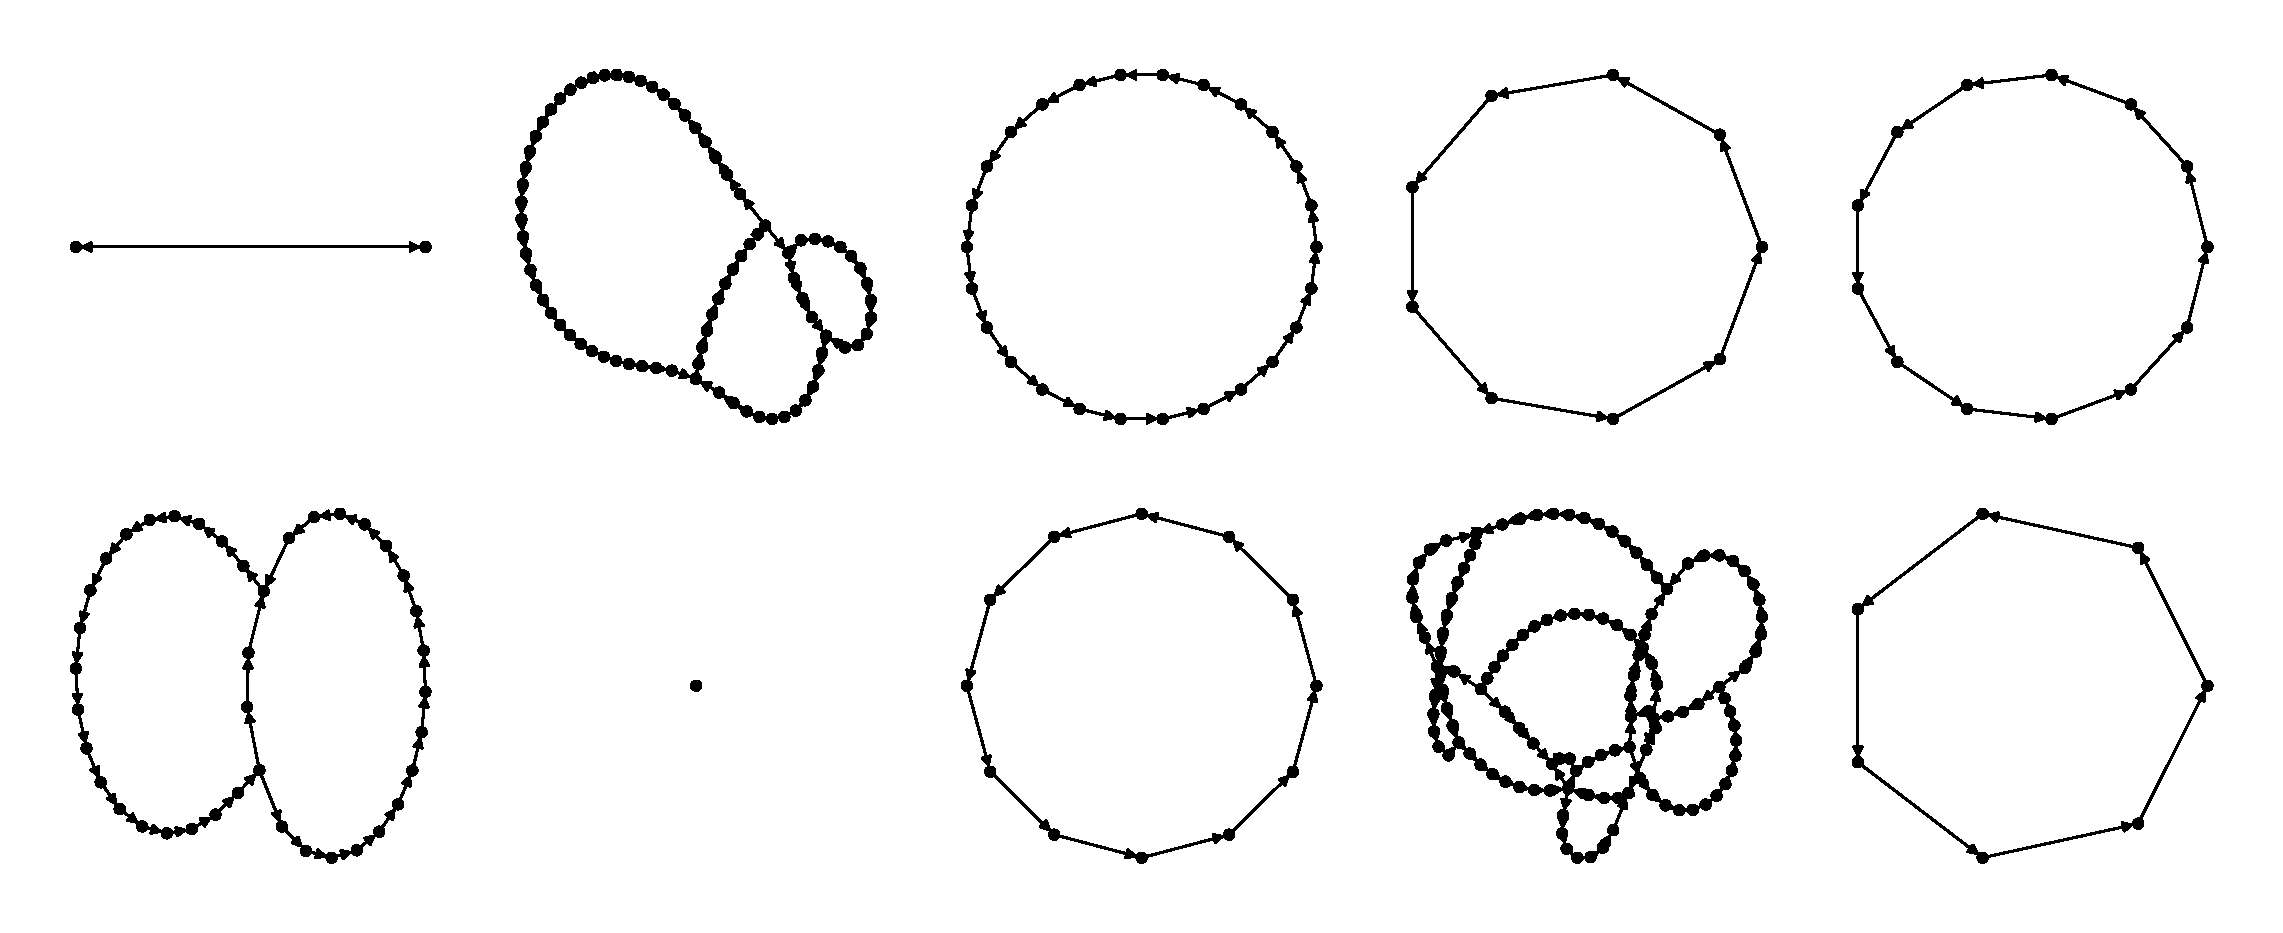
\includegraphics[width=\textwidth]{Content/Pictures/largest_sccs.eps}
    
    \caption{The largest SCC from samples of a directed configuration model with independent $\text{Poisson(1)}$ in- and out-degrees}
    \label{fig:largest-sccs}
\end{figure}

In \cref{fig:largest-sccs} \myworries{actually generate sccs from a poisson model} we see the largest SCC from samples of a directed configuration model. As can be seen, while the lengths of paths in the SCC are long, the actual structure of the SCC is often quite simple. In some cases the largest SCC is just a single cycle.  This was confirmed in previous work by \myworries{insert reference for DER}. There it was shown that while the lengths of paths in the SCC will scale like $n^{1/3}$, the actual structure of the SCC will remain finite.

To formalise this idea we will introduce metric directed multigraphs (MDMs). These are simply weighted directed multigraphs, but in our context it is more appropriate to think of the weights as lengths hence the change in naming. Formally a directed multigraph is a tuple $M = (V, E, r)$ where

\subsection{Previous work}


\subsection{Proof outline}
The techniques we will use to investigate the graph model are a combination of the techniques introduced by Conchon-Kerjan and Goldschmidt in \cite{Conchon2018} and the strategy of Goldschmidt and Stephenson in \cite{Goldschmidt2019}. The former work discusses the scaling limit of an undirected uniform graph with i.i.d.\ degrees at criticality, and the latter discusses the scaling limit of the strongly connected components of a directed Erd\H{o}s-Renyi graph at criticality.\\
To investigate the structure of the strongly connected components of a uniform graph with degree sequence $(\mathbf{D}_1,\dots,\mathbf{D}_n)$, conditioned on $\sum_{i=1}^n D^-_i=\sum_{i=1}^n D^+_i$, we will use a version of the configuration model for digraphs that was introduced in \cite{Cooper2004}. The output of the configuration model, conditioned on being a simple graph, is a uniform digraph with the given degree sequence. \\
\myworries{Description of exploration written by Zheneng} This is illustrated in Figure \ref{fig.configuration model}. 
\begin{figure}
    \centering
    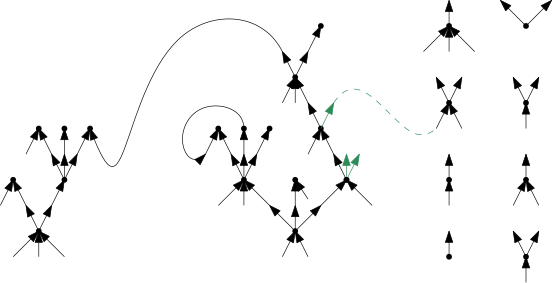
\includegraphics[scale=0.6]{Content/Pictures/Configuration model.png}
    \caption{The green arrows represent unpaired out-half-edges of vertices that have been visited. One by one, in depth first order, these are paired to a uniform unpaired in-half-edge.}
    \label{fig.configuration model}
\end{figure}\\
The exploration algorithm naturally gives rise to a forest that we will refer to as the \emph{out-forest}, which will play a key role in studying the limit under rescaling of the strongly connected components. An important motivation for studying the out-forest is the fact that the vertex set of any strongly connected component is contained in one of the components of the out-forest. We define the out-forest in such a way that every time step in the exploration corresponds to one vertex in the out-forest. At every time step in the exploration at which we find an unseen vertex, say with out-degree $d^+$, we add a vertex with $d^+$ children to the out-forest. At every time step at which we do not find a new vertex, but instead connect to a previously found vertex, we add a purple leaf to the out-forest. This is illustrated in Figure \ref{fig.configuration modeloutforest}. We refer to the out-forest corresponding to the exploration up to time $k$ as $\hat{\cF}_n(k)$.\\
A key fact is that the out-forest can be sampled without knowing what the endpoints of the surplus edges are, because this information does not affect the law of the out-forest. This allows us to build up the randomness of the exploration in the following layers.
\begin{enumerate}
    \item We sample the out-forest $(\hat{\cF}_n(k),k\geq 1)$. 
    \item We visit the purple vertices in $(\hat{\cF}_n(k),k\geq 1)$, and for each vertex we sample whether it is the starting point of a \emph{candidate}, i.e. whether the corresponding surplus edge is possibly part of a strongly connected component.
    \item We visit the starting points of the candidates in depth-first order, and for each of them, sample where the endpoint of the corresponding surplus edge is.
\end{enumerate}

\begin{figure}
    \centering
    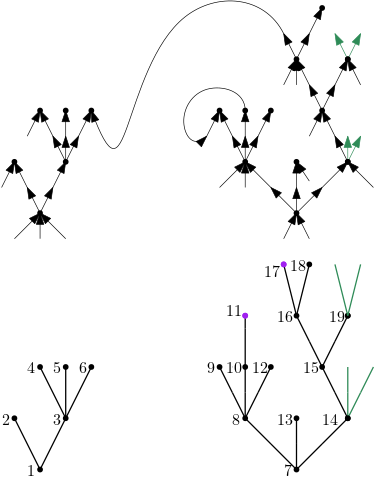
\includegraphics[scale=0.8]{Content/Pictures/Configuration model out-forest.png}
    \caption{The out-forest is defined based on the exploration of the digraph. For each surplus edge, we add an extra leaf, which we colour purple. The labels of the vertices correspond to the time step in the exploration at which the vertex is added. The green edges lead to vertices of which the degree and colour have not yet been sampled.}
    \label{fig.configuration modeloutforest}
\end{figure}
Then, our approach is as follows.
\begin{enumerate}
    \item We find the limit under rescaling of $\hat{\cF}_n(m_n)$ for $m_n=O(n^{2/3})$ conditional on $\sum_{i=1}^n D^-_i=\sum_{i=1}^n D^+_i$ and simplicity of the digraph. We do this by studying the height process and \L ukasiewicz path of the out-forest.
    \item We show that the positions of the candidates converge.
    \item We can recover the strongly connected components that appear in the exploration up to time $m_n$ from  $\hat{\cF}_n(m_n)$ and the positions of the candidates up to time $m_n$. We do this by making vertex identifications and performing a cutting procedure. We show that these procedures carry over to the limit.
    \item We show that for any $\delta>0$, with high probability, all strongly connected components with length larger than $\delta n^{1/3}$ are contained in the exploration up to time $O(n^{2/3})$. Therefore, we can choose $m_n$ such that, with high probability, we do not miss any large strongly connected components by only considering the exploration up to time $m_n$. This finishes the proof of the convergence in the product topology.
\end{enumerate}

